\chapter*{Scenari operativi}
I possibili casi d’uso del sistema sono:
\begin{itemize}
\item \textbf{Aula:} che può essere \textit{agibile} o \textit{non agibile}
\item \textbf{Gomp:}  può essere, come ogni sistema informatico, \textit{operativo} o \textit{non operativo}.
\item \textbf{Prodigit:} anche in questo caso ha la possibilità di essere \textit{operativo} o \textit{non operativo}, ma ciò dipende dallo stato del Gomp. Sebbene il sistema, per un certo periodo di tempo possa funzionare in modo autonomo necessita comunque delle informazioni fornitegli dal Gomp, nel caso in cui non sia operativo ovviamente non può essere effettuata nessuna azione con esso.
\item \textbf{Studente:} ha due casi possibili, o usa Prodigit o non può fare nulla perché non autorizzato, in questo modo si modella la turnazione delle matricole come richiesto dalla specifica, ovvero ogni settimana si ha metà degli studenti che possono prenotare un posto e metà che non possono.
Se lo studente ha la possibilità di interfacciarsi con Prodigit allora decide se effettuare una prenotazione e quindi occupare un posto dell’aula, oppure cancellare una prenotazione e quindi liberare un posto.
\end{itemize}

Il sistema nel suo complesso è verosimile e robusto,  ciò è verificabile facendo diversi esperimenti variando  alcuni parametri. \\
Si esegue quindi il sistema considerando alcuni casi estremi, per esempio nel caso in cui lo studente effettua solo prenotazioni si otterrà un grafico come in figura~\ref{figura: solo prenotazioni}.


\begin{figure}[htp]
\begin{center}
  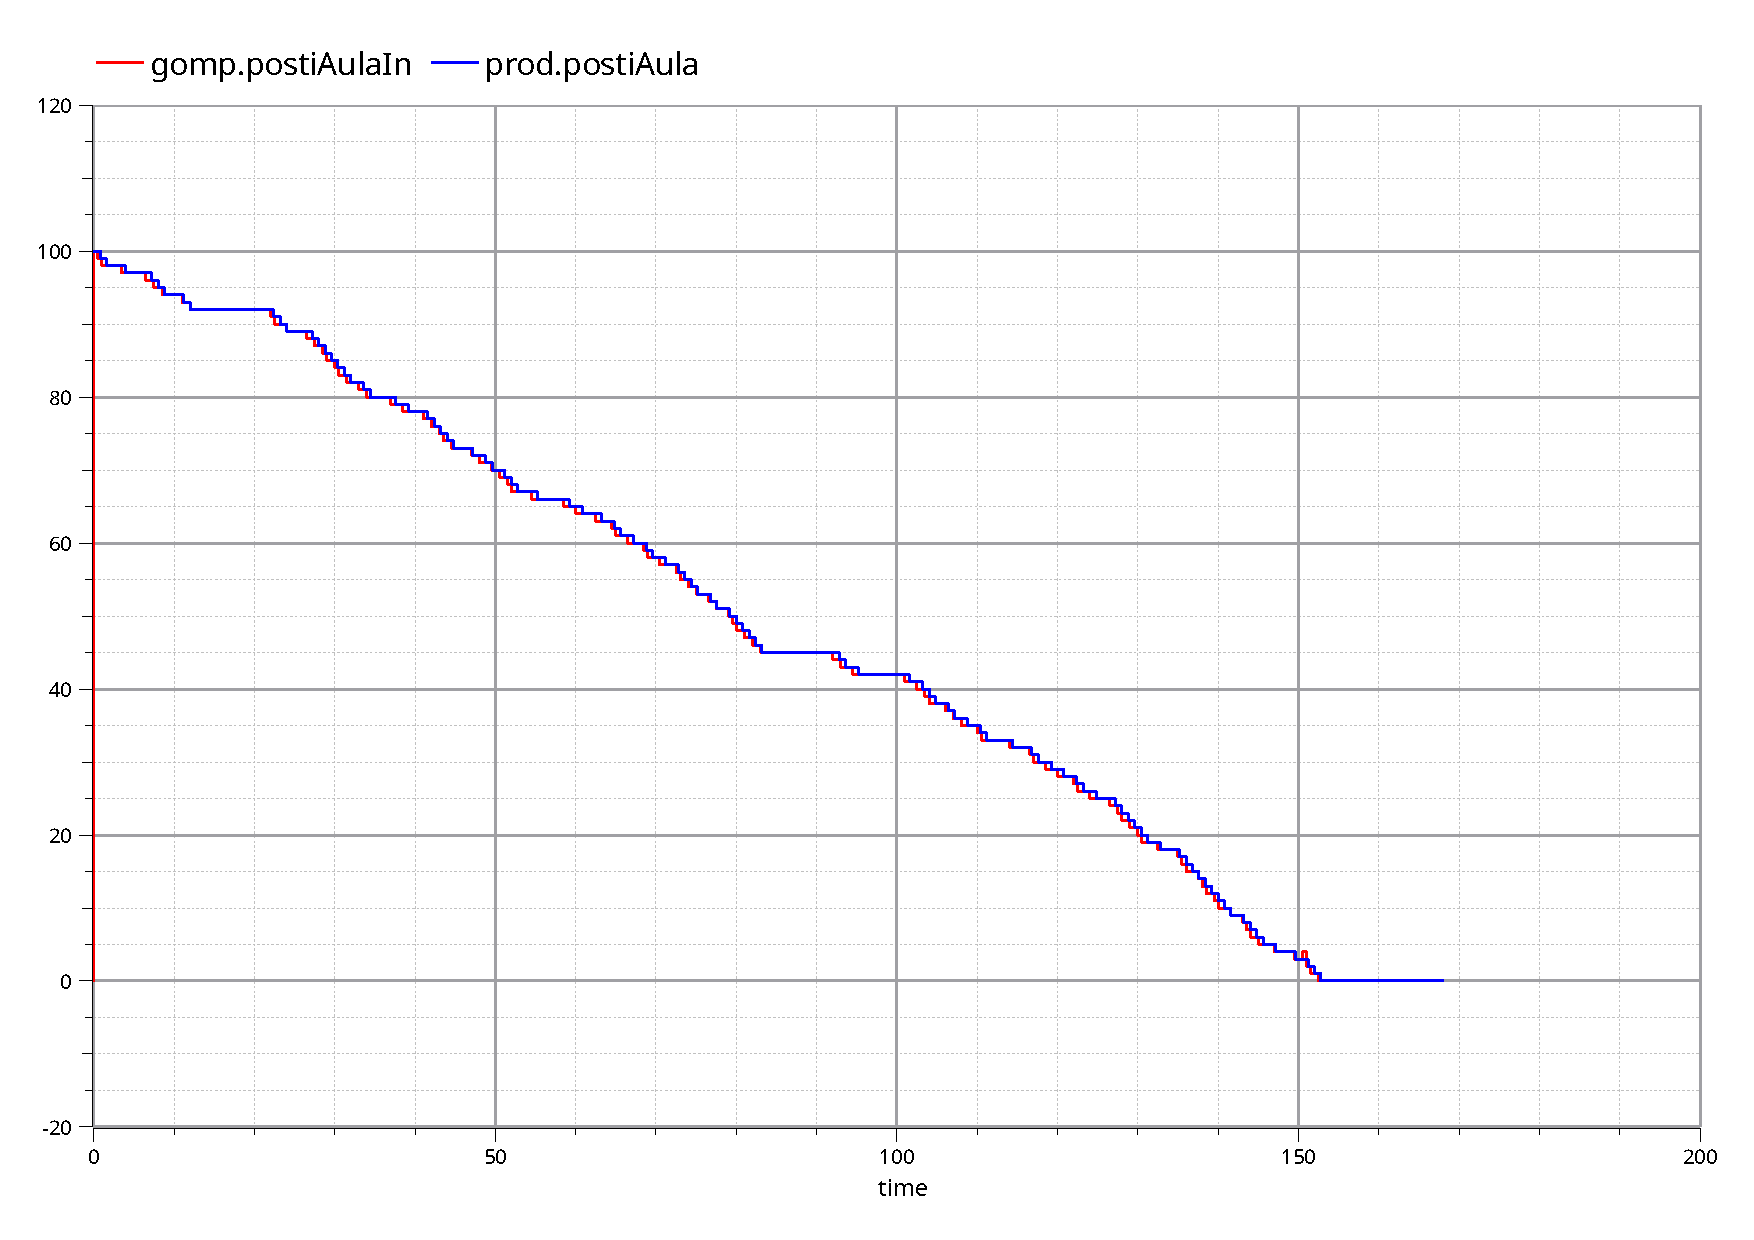
\includegraphics[width=1 \textwidth]{Figure/studente solo prenotazioni.pdf}
    \caption{Grafico che mostra l’andamento dei posti nell’aula nel caso estremo in cui siano presenti solo prenotazioni, è utile notare  l’ultima parte del grafico che rimane costante al valore 0 fino alla fine della simulazione.} \label{figura: solo prenotazioni}
\end{center}
\end{figure}

Nel caso opposto (ovvero con solo cancellazioni) a quello mostrato in figura si otterrà una linea costante.\\

Un altro caso estremo che si può considerare è quello in cui Prodigit è sempre non raggiungibile e quindi non si ha la possibilità di effettuare nessuna azione, ciò è visibile dal grafico nella figura ~\ref{figura:prodigit down}, in cui è evidente che i posti dell’aula rimangono  costanti al valore iniziale.

\begin{figure}[htp]
\begin{center}
  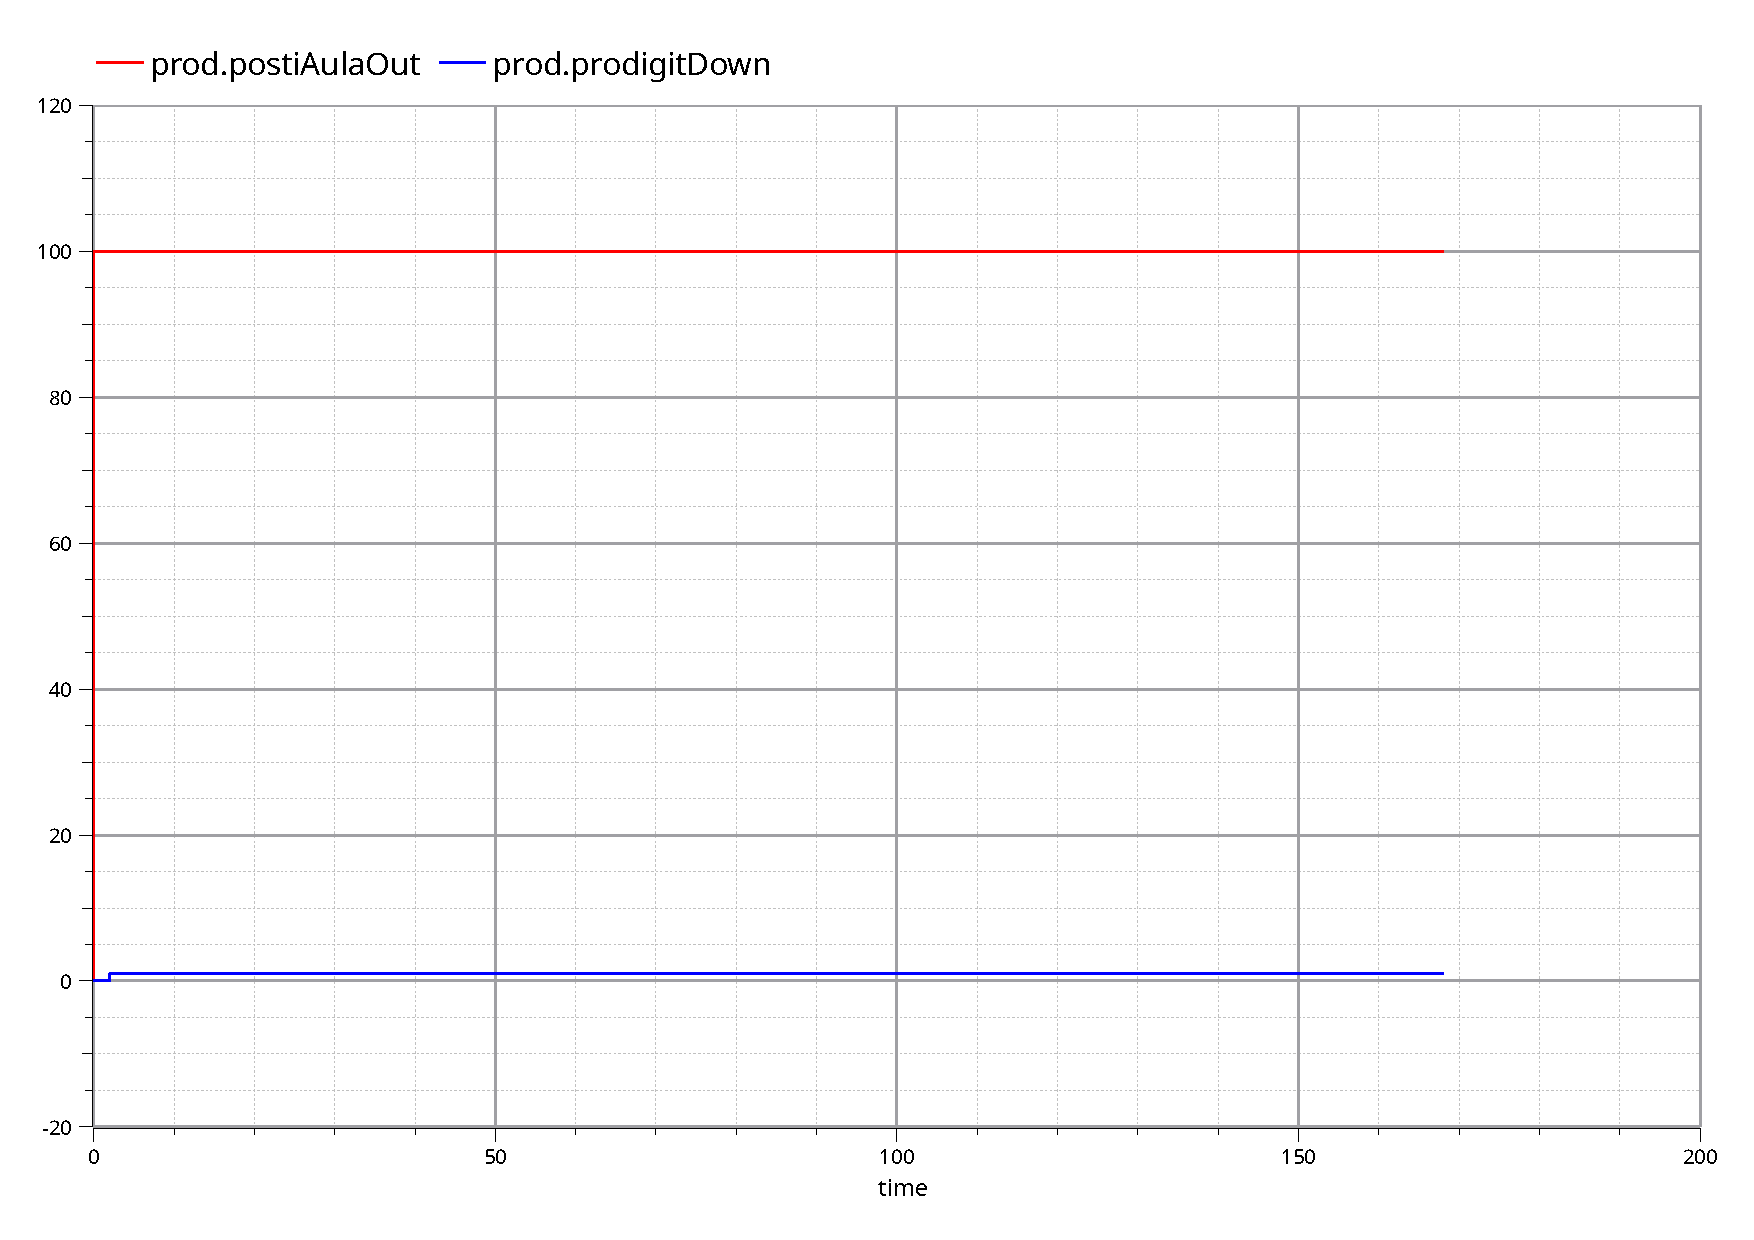
\includegraphics[width=1 \textwidth]{Figure/posti prod down.pdf}
    \caption{Grafico che rappresenta il caso in cui Prodigit è costantemente down, l’andamento della variazione dei posti  è costante al valore iniziale.}\label{figura:prodigit down}
\end{center}
\end{figure}

